\documentclass [10pt]{article}
\textheight	8.7in
\textwidth	6.5in
\topmargin	    0in
\oddsidemargin  0in
\evensidemargin 0in
\baselineskip 15pt

\usepackage{amssymb,amsmath,amstext}
\usepackage{amsfonts}
\usepackage{mathtools}
\usepackage{tikz}
\usetikzlibrary{automata,arrows,calc,positioning}

\begin{document}
\title{Theory of Computation Assignment no. 4}
\author{Goktug Saatcioglu}
\date{}
\maketitle

\begin{enumerate}
	\item[\textbf{(1)}]
	\begin{enumerate}
		\item[a.]Assume for the sake of contradiction that $A$ is regular. Then $A$ has a pumping constant $p$. Now consider the word $a^{p}b^{p}c^{2p}$ (i.e. there are $p$ $a$'s and $b$'s and $2p$ $c$'s). Then we can write $w$ as $w = xyz$ such that the properties of the pumping lemma hold. By the properties that states that $\left|xy\right| \le p$ and $\left|y\right| > 0$, we can conclude that $y$ consists of only $a$'s (so does $xy$). By the property $xy^{n}z \in A\:\:\forall n \ge 0$, there exists a $w^{\prime} = xy^{2}z$ such that $w^{\prime} \in A$. However, since $\left|xy\right| \le p$ and $\left|y\right| \ge 0$ there are now at least $p + 1$ $a$'s but we also still have $p$ $b$'s and $2p$ $c$'s. Therefore, for $w^{\prime}$ $\#a(w^{\prime}) + \#b(w^{\prime}) > \#c(w^{\prime})$ and $w^{\prime} \notin A$. This is a contradiction to our initial claim that $A$ is regular and we conclude that $A$ is not regular.
		\item[b.]Assume for the sake of contradiction that $B$ is regular. Then $B$ has a complement $B^{\prime}$ such that $B^{\prime}$ is regular by the closure properties of regular languages. Define$$B^{\prime} = \{w\in\{a,b,c\}^{*}\:|\:\#a(w)\le\#b(w)\land\#a(w)\ge\#c(w)\},$$using De Morgan's Law. If $B^{\prime}$ is regular then $B^{\prime}$ has a pumping constant $p$. Now consider the word $w=a^{p}b^{p}c^{p}$ (i.e. there are $p$ $a$'s, $b$'s and $c$'s). We can write $w$ as $w=xyz$ such that the properties of the pumping lemma hold. By the properties that states that $\left|xy\right| \le p$ and $\left|y\right| > 0$, we can conclude that $y$ consists of only $a$'s (so does $xy$). By the property $xy^{n}z \in B^{\prime}\:\:\forall n \ge 0$, there exists a $w^{\prime} = xy^{2}z$ such that $w^{\prime} \in B^{\prime}$ and there also exists a $w^{\prime\prime} = xy^{0}z$ such that $w^{\prime\prime} \in B^{\prime}$. We know that $w^{\prime}$ consists of at least $p+1$ $a$'s while $w^{\prime\prime}$ consists of at most $p-1$ $a$'s. For $w^{\prime}$, $\#a(w)>\#b(w)$ meaning $w^{\prime} \notin B^{\prime}$ and for $w^{\prime\prime}$, $\#a(w)<\#c(w)$ meaning $w^{\prime\prime} \notin B^{\prime}$. (Note: We used $w^{\prime}$ and $w^{\prime\prime}$ to demonstrate more than one way of doing this proof, one of them is sufficient.) We get a contradiction to our claim that $B^{\prime}$, which is the complement of $B$, is regular. This is in turn a contradiction to our initial claim that $B$ is regular and conclude that $B$ is not regular.
		\item[c.]Assume for the sake of contradiction that $C$ is regular. Then $C$ has a pumping constant $p$. Now consider the word $a^{p^{2}}$ (i.e. there are $p^{2}$ $a$'s). Then we can write $w$ as $w = xyz$ such that the properties of the pumping lemma hold. By the properties that states that $\left|xy\right| \le p$ and $\left|y\right| > 0$, we can conclude that $y$ consists of only $a$'s (so does $xy$). This is because $a^{p^{2}}=a^{p}a^{p}$. By the property $xy^{n}z \in C\:\:\forall n \ge 0$, there exists a $w^{\prime} = xy^{2}z$ such that $w^{\prime} \in C$. Since $\left|xy\right| \le p \implies \left|y\right| \le p$ and $\left|y\right| > 0$, we know that $p^{2} < \left|xy^{2}z\right| < p^{2}+p$. However, $p^{2}+p<p^{2}+2p+1=(p+1)^{2}$ meaning that $\left|xy^{2}z\right|$ lies strictly between the two consecutive perfect squares $p^{2}$ and $(p+1)^{2}$. Thus, the length of $w^{\prime}$ is not a perfect square and $w^{\prime} \notin C$. This is a contradiction to our initial claim that $C$ is regular and we conclude that $C$ is not regular.
	\end{enumerate}
	\item[\textbf{(2)}]Assume for the sake of contradiction that $D$ is regular. Then $D\setminus D^{\prime} = D^{\prime\prime}$ where $D^{\prime}$ is also regular should give us another regulare language by the closure properties of regular languages. Define $$D^{\prime}=\{w\in\{a,b\}^{*}\:|\:\text{no three consecutive letters are the same}\}.$$$D^{\prime}$ is regular since there exists a DFA or NFA that identifies it. From the definition of $D$,$$D^{\prime\prime}=\{w\in\{a,b\}^{*}\:|\:\#a(w)=\#b(w)\}.$$ If $D^{\prime\prime}$ is regular then $D^{\prime\prime}$ has a pumping constant $p$. Now consider the word $w=a^{p}b^{p}$ (i.e. there are $p$ $a$'s and $b$'s). We can write $w$ as $w=xyz$ such that the properties of the pumping lemma hold. By the properties that states that $\left|xy\right| \le p$ and $\left|y\right| > 0$, we can conclude that $y$ consists of only $a$'s (so does $xy$). By the property $xy^{n}z \in D^{\prime\prime}\:\:\forall n \ge 0$, there exists a $w^{\prime} = xy^{2}z$ such that $w^{\prime} \in D^{\prime\prime}$. However, since $y$ consists of at least one $a$, there are now at least $p + 1$ $a$'s but we also still have $p$ $b$'s. For $w^{\prime}$, $\#a(w)>\#b(w)$ meaning $w^{\prime} \notin D^{\prime\prime}$ which gives us a contradiction. Thus, $D^{\prime\prime}$ is not regular and we then get a contradiction to our initial claim that $D$ was regular. We conclude that $D$ is not regular.
	\item[\textbf{(3)}]
	\begin{enumerate}
		\item[a.]The language $F$ is regular since it is very easy to create a DFA that identifies it. On the other hand, the language $E$ is not regular. Assume for the sake of contradiction that $E$ is regular. Then $E$ has a pumping constant $p$. Now consider the word $(ab)^{p}c(ab)^{p}$ (i.e. there are $2p$ $ab$'s and $1$ $c$). Then we can write $w$ as $w = xyz$ such that the properties of the pumping lemma hold. By the properties that states that $\left|xy\right| \le p$ and $\left|y\right| > 0$, we can conclude that $y$ consists of only $b$'s if $\left|y\right|=1$ and $ab$'s if $1 < \left|y\right|\le p$ (similarly $xy$ consists of only $a$'s if $\left|x\right|=1$, $ab$'s if $1 < \left|x\right| < p$ and $\lambda$ if $\left|x\right|=0$). By the property $xy^{n}z \in E\:\:\forall n \ge 0$, there exists a $w^{\prime} = xy^{2}z$ such that $w^{\prime} \in C$. After pumping, the $xy$ pair will contain more $ab$'s than the $ab$'s in $z$ if $y$ contains at least a single $ab$. Furthermore, if $y$ only contains a single $b$, then the $(ab)^{p}c(ab)^{p}$ property will not hold. Thus, $w^{\prime} \notin E$and we get a contradiction to our initial claim that $E$ is regular. Thus, we conclude that $E$ is not regular.\\
		Yet, we can arbitrarily pump the any $a$ or $b$ in the language $F$ to satisfy the requirement that there is either an $aa$ or $bb$. Again consider the word $(ab)^{p}c(ab)^{p}$. Then we can write $w$ as $w = xyz$ such that the properties of the pumping lemma hold. By the properties that states that $\left|xy\right| \le p$ and $\left|y\right| > 0$, we can conclude that if $y$ consists of more $b$'s than $a$'s then we can obtain $bb$ as a substring (this means that $b$, $bab$, $babab$ and so on is necessary). Furthermore, note that it is impossible to obtain more $a$'s than $b$'s for $y$ and if we have an equal number of $a$'s and $b$'s it is not possible to obtain $bb$ as a substring. In this case we must have $\left|y\right| = 1 + i \le p$ where $i = 2,4,6,..$ (even numbers) and $\left|xy\right| = p - \left|y\right|$. By the property $xy^{n}z \in G\:\:\forall n \ge 0$, there exists a $w^{\prime} = xy^{2}z$ such that $w^{\prime} \in G$. After pumping, we are gauranteed to at least have one substring that is $bb$ . In fact, we can generalize our argument to all $n>1$ since we will pump a substring so that we are guaranteed to see an $bb$. Thus, we must find cases for $n=0$ and $n=1$ such that the pumping property also holds. For $n=0$ consider the word $(ab)^{p-1}c(ab)^{p-1}$ so that we can select $y=c$ and pump out $c$ to obtain the substring $bb$. For $n=1$ consider any word $aa^{p}bb^{p}$ and pumping with $n=1$ (or any other $n$ making this a trivial solution) will satisfy the pumping property. This last word works because we construct $G$ using $E\bigcup F$. Thus, for all cases we see that $w^{\prime} \in F$ which in turn means that $w^{\prime} \in G$. Thus, $G$ has the pumping property.
		\item[b.]$G$ should not be a regular language because, intuitively, there would need to exist a DFA that recognizes an $n$ amount of $ab$'s and after seeing a $c$ recognize an additional $n$ amount of $ab$'s. This implies that we need an unbounded amount of memory in order to recognize $n$ and the language specified by $E$ (which is contained in the union of $E$ and $F$). Since regular languages are languages which can be recognized by an automaton with a fixed amount of memory, $E$ is not regular. (Note: A rigorous proof of why $E$ is not regular using the pumping lemma is given above in (a).) However, the union of $E$ and $F$ will require us to count the values occuring in $E$ in some way to include the language of $E$. Furthermore, $E$ is expressed in the form of $(ab)^{n}c(ab)^{n}$ where $n\ge0$ meaning that $E$ will never contain the substring $aa$ or $bb$ (which is the language $F$). We can possibly detect if an arbitrary $aa$ or $bb$ but we would need to remember that detection going forward. Thus, $G$ should not be a regular language.
		\item[c.]We can use the Myhill-Nerode theorem to prove that $G \notin REG$. $G$ contains infinitely many words. Let's pick two words, $w_{1}$ and $w_{2}$ that are in $G$ and $w_{1} \ne w_{2}$. These words are defined by the union of the languages of $E$ and $F$. Now notice that there are infinitely many ways to distinguish $w_{1}$ and $w_{2}$ (one such way is to keep padding either $a$'s or $b$'s). Therefore, by the Myhill-Nerode theorem, $G \notin Reg$.
	\end{enumerate}
	\item[\textbf{(4)}]
	\begin{enumerate}
		\item[i.]$a^{*}(ba^{*}ba^{*})^{*}$
		\item[ii.]$(bb^{*}a)^{*}(\lambda \lor bb^{*})$
		\item[iii.]$(a^{*}(ba)^{*})^{*}(\lambda \lor b)$
	\end{enumerate}
	\item[\textbf{(5)}]
	\begin{enumerate}
		\item[i.]
		\begin{enumerate}
			\item[(a)]Below is the NFA that recognizes the language $K = \{ba,bab\}^{*}$.\\
			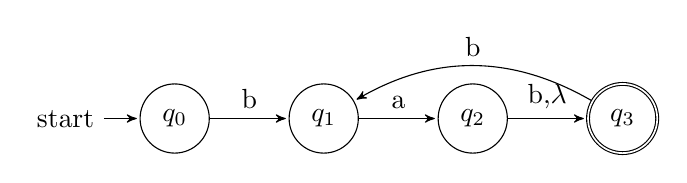
\begin{tikzpicture}[baseline=(q_0.north),>=stealth',shorten >=1pt, auto,node distance=1cm,align=center]
				\node[state,initial] (q_0) {$q_0$};
				\node[state] [right=of q_0] (q_1) {$q_1$};
				\node[state] [right=of q_1] (q_2) {$q_2$};
				\node[state,accepting] [right=of q_2] (q_3) {$q_3$};
				\path[->]
					(q_0) edge node {b} (q_1)
					(q_1) edge node {a} (q_2)
					(q_2) edge node {b,$\lambda$} (q_3)
					(q_3) edge [bend right] node [above] {b} (q_1);
			\end{tikzpicture}
			\\Where $q_{0}$ is the empty string $\lambda$, $q_{1}$ is $\{b,bab,babb\}^{*}$, $q_{2}$ is $\{ba^{*}\lor bab^{*}\}$ (will not recognize $K$) and $q_{3}$ is $\{ba,bab\}^{*}$.
			\item[(b)]The conversion of the NFA to a DFA is below.\\
			\begin{tikzpicture}[baseline=(q_0.north),>=stealth',shorten >=1pt, auto,node distance=1cm,align=center]
				\node[state,initial] (q_0) {$q_{0}^{\prime}$};
				\node[state] [right=of q_0] (q_1) {$q_{1}^{\prime}$};
				\node[state,accepting] [right=of q_1] (q_2) {$q_{2}^{\prime}$};
				\node[state,accepting] [right=of q_2] {$q_{3}^{\prime}$};
				\path[->]
					(q_0) edge node {b} (q_1)
					(q_1) edge node {a} (q_2)
					(q_2) edge node {b} (q_3)
					(q_3) edge [bend right] node [above] {b} (q_1)
					(q_3) edge [bend left] node [below] {a} (q_2);
			\end{tikzpicture}
			\\Where $q_{0}^{\prime} = \{q_{0}\}$, $q_{1}^{\prime} = \{q_{1}\}$, $q_{2}^{\prime} = \{q_{2},q_{3}\}$ and $q_{3}^{\prime} = \{q_{1},q_{3}\}$. States that are not denoted by prime are defined above in (a).
		\end{enumerate}
	\end{enumerate}
	\item[\textbf{(6)}]The steps to finding a regular expression for the language described by the automaton are displayed below.\\
	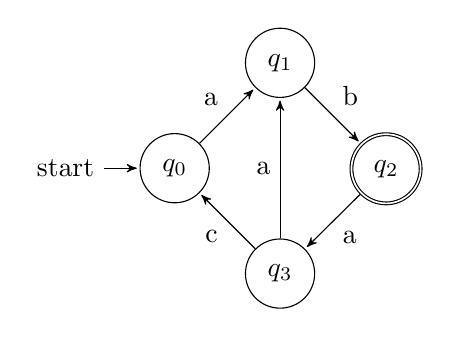
\begin{tikzpicture}[baseline=(q_0.north),>=stealth',shorten >=1pt, auto,node distance=1cm,align=center]
		\node[state,initial] (q_0) {$q_{0}$};
		\node[state] [above right=of q_0] (q_1) {$q_{1}$};
		\node[state] [below right=of q_0] (q_3) {$q_{3}$};
		\node[state,accepting] [below right=of q_1] (q_2) {$q_{2}$};
		\path[->]
			(q_0) edge node {a} (q_1)
			(q_1) edge node {b} (q_2)
			(q_2) edge node {a} (q_3)
			(q_3) edge node {a} (q_1)
			(q_3) edge node {c} (q_0);
	\end{tikzpicture}\\
	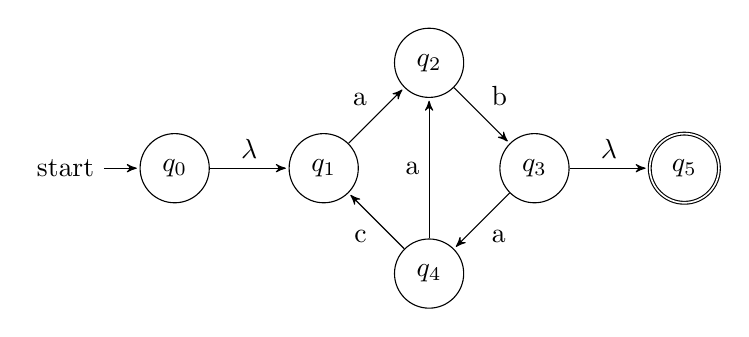
\begin{tikzpicture}[baseline=(q_0.north),>=stealth',shorten >=1pt, auto,node distance=1cm,align=center]
		\node[state,initial] (q_0) {$q_{0}$};
		\node[state] [right=of q_0] (q_1) {$q_{1}$};
		\node[state] [above right=of q_1] (q_2) {$q_{2}$};
		\node[state] [below right=of q_1] (q_4) {$q_{4}$};
		\node[state] [below right=of q_2] (q_3) {$q_{3}$};
		\node[state,accepting] [right=of q_3] (q_5) {$q_{5}$};
		\path[->]
			(q_0) edge node {$\lambda$} (q_1)
			(q_1) edge node {a} (q_2)
			(q_2) edge node {b} (q_3)
			(q_3) edge node {a} (q_4)
			(q_4) edge node {a} (q_2)
			(q_4) edge node {c} (q_1)
			(q_3) edge node {$\lambda$} (q_5);
	\end{tikzpicture}\\
	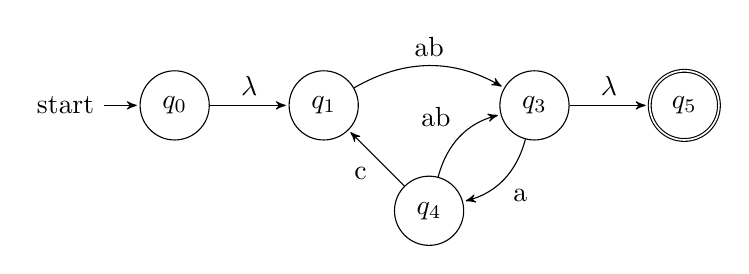
\begin{tikzpicture}[baseline=(q_0.north),>=stealth',shorten >=1pt, auto,node distance=1cm,align=center]
		\node[state,initial] (q_0) {$q_{0}$};
		\node[state] [right=of q_0] (q_1) {$q_{1}$};
		\node[state] [below right=of q_1] (q_4) {$q_{4}$};
		\node[state] [above right=of q_4] (q_3) {$q_{3}$};
		\node[state,accepting] [right=of q_3] (q_5) {$q_{5}$};
		\path[->]
			(q_0) edge node {$\lambda$} (q_1)
			(q_1) edge [bend left] node {ab} (q_3)
			(q_3) edge [bend left] node {a} (q_4)
			(q_4) edge [bend left] node {ab} (q_3)
			(q_4) edge node {c} (q_1)
			(q_3) edge node {$\lambda$} (q_5);
	\end{tikzpicture}\\
	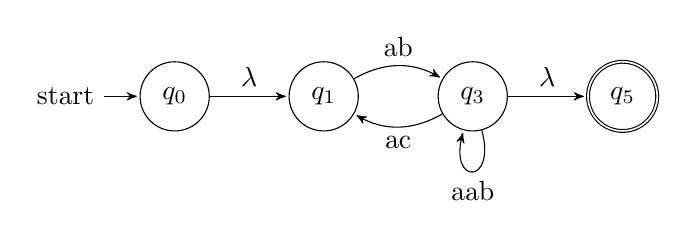
\begin{tikzpicture}[baseline=(q_0.north),>=stealth',shorten >=1pt, auto,node distance=1cm,align=center]
		\node[state,initial] (q_0) {$q_{0}$};
		\node[state] [right=of q_0] (q_1) {$q_{1}$};
		\node[state] [right=of q_1] (q_3) {$q_{3}$};
		\node[state,accepting] [right=of q_3] (q_5) {$q_{5}$};
		\path[->]
			(q_0) edge node {$\lambda$} (q_1)
			(q_1) edge [bend left] node {ab} (q_3)
			(q_3) edge [bend left] node {ac} (q_1)
			(q_3) edge [loop below] node {aab}
			(q_3) edge node {$\lambda$} (q_5);
	\end{tikzpicture}\\
	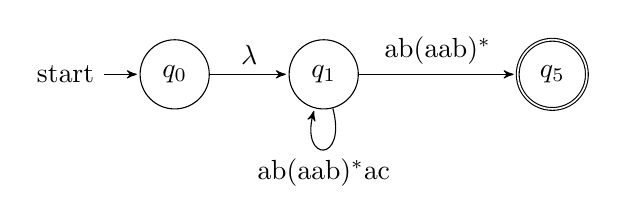
\begin{tikzpicture}[baseline=(q_0.north),>=stealth',shorten >=1pt, auto,node distance=1cm,align=center]
		\node[state,initial] (q_0) {$q_{0}$};
		\node[state] [right=of q_0] (q_1) {$q_{1}$};
		\node[state,accepting] [right=2cm of q_1] (q_5) {$q_{5}$};
		\path[->]
			(q_0) edge node {$\lambda$} (q_1)
			(q_1) edge [loop below] node {ab(aab)$^{*}$ac} (q_5)
			(q_1) edge node {ab(aab)$^{*}$} (q_5);
	\end{tikzpicture}\\
	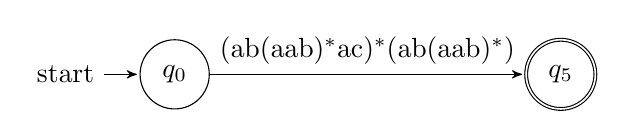
\begin{tikzpicture}[baseline=(q_0.north),>=stealth',shorten >=1pt, auto,node distance=1cm,align=center]
		\node[state,initial] (q_0) {$q_{0}$};
		\node[state,accepting] [right=4cm of q_0] (q_5) {$q_{5}$};
		\path[->]
			(q_0) edge node {(ab(aab)$^{*}$ac)$^{*}$(ab(aab)$^{*}$)} (q_5);
	\end{tikzpicture}\\
	Therefore, the regular expression for the language described by this automaton is $(ab(aab)^{*}ac)^{*}(ab(aab)^{*})$.
	\item[\textbf{(7)}]We need to prove that if $r$ is a regular expression, then there exists $L(r) \in REG$. We prove this by showing that for $r$ there exists an NFA that recognizes the language of $r$, i.e. $L(r) = L(N_{r})$.\\
	Our base case involves proving for the base cases for regular expressions that there exists a NFA that identifies them. These base cases are: $\phi$ (the empty set), $\lambda$ (the language containing the empty string alone, $\{\lambda\}$) and $a$ (the language containing a single letter, $\{a\}$). For a previous homework assignment we have proved that a DFA exists for each of these base cases. Since a DFA exists for each of these cases, we can say that an NFA also exists that identifies each of these languages (the automaton have not been drawn here but such proofs were given in the answers to HW2 and it is trivial to prove the existence of such automaton).\\
	Now we move onto the inductive step. We know that we can construct larger regular expressions from our base regular expressions using the $\bigcup$, $\cdot$ and $^{*}$ operators. Consider an $r$ that is recursively defined by our operators such that $r_{1}$ and $r_{2}$ are regular expressions that compose $r$. Since we proved that there exists NFAs that identify our base regular expressions and we know that there exists NFAs that identify the $\bigcup$, $\cdot$ and $^{*}$ (such constructions are also regular and the proofs for this are in the lecture notes), we can build an $r_{1}$ and $r_{2}$ that serves as an induction hypothesis and there exists an NFA that identifies the language $L(r)$.\\
	Thus, we prove the existence of $L(r) = L(N_{r})$. Since $L(N_{r})$ exists and a language, by definition, is regular if there exists an NFA that identifies it, we can say that $L(r) \in REG$. Then this proof applies for all regular expressions $r$ since we can construct an NFA that recognizes the language of $r$ which then implies $L(r) \in REG$.
\end{enumerate}

\end{document}